\documentclass[aspectratio=169, 10pt]{beamer}
\usepackage{bbm}
%\usepackage{algorithm2e}
%\usepackage{mathtools}
%\usepackage{graphicx}
%\usepackage{animate}
%\usepackage{hyperref}
\renewcommand\appendixname{Appendix}
%\usepackage{xcolor}
\usepackage[customcolors]{hf-tikz}
%\tikzset{offset def/.style={
%        above left offset={-0.1,0.35},
%        below right offset={0.1,-0.2},
%    },
%    color def/.style={
%        offset def,
%        set fill color=green,
%        set border color=red,
%    },
%}
\usepackage{marvosym}
\usepackage{fontawesome}
\colorlet{rred}{red!80!black}
\colorlet{ggreen}{green!80!black}
\colorlet{grey}{black!50!white}

\usetheme[progressbar=foot]{metropolis}
\metroset{block=fill}
\usepackage{appendixnumberbeamer}
\setbeamercovered{invisible}

\usepackage{booktabs}
\usepackage[scale=2]{ccicons}
\usepackage[style=authortitle,backend=bibtex]{biblatex}
\addbibresource{biblio.bib}

\usepackage{pgfplots}
\usepgfplotslibrary{dateplot}
\setbeamertemplate{caption}{\raggedright\insertcaption\par}
\setlength{\abovecaptionskip}{-3pt plus 0pt minus 0pt}

%\usepackage{xspace}
\theoremstyle{definition}
\newtheorem{defn}{Definition}
\newtheorem{obs}{Observation}

% math symbols
% Fancy math fonts, requires amsfonts and amsmath
%% Elephant Letters
\newcommand{\A}{\mathbb{A}}
\newcommand{\B}{\mathbb{B}}
\newcommand{\Ch}{\mathbb{C}}
\newcommand{\D}{\mathbb{D}}
\newcommand{\E}{\mathbb{E}}
\newcommand{\F}{\mathbb{F}}
\newcommand{\Gh}{\mathbb{G}}
\newcommand{\Hh}{\mathbb{H}}
\newcommand{\I}{\mathbb{I}}
\newcommand{\J}{\mathbb{J}}
\newcommand{\K}{\mathbb{K}}
\newcommand{\Lh}{\mathbb{L}}
\newcommand{\M}{\mathbb{M}}
\newcommand{\N}{\mathbb{N}}
\newcommand{\Oh}{\mathbb{O}}
\newcommand{\Ph}{\mathbb{P}}
\newcommand{\Q}{\mathbb{Q}}
\newcommand{\R}{\mathbb{R}}
\newcommand{\Sh}{\mathbb{S}}
\newcommand{\T}{\mathbb{T}}
\newcommand{\Uh}{\mathbb{U}}
\newcommand{\V}{\mathbb{V}}
\newcommand{\W}{\mathbb{W}}
\newcommand{\X}{\mathbb{X}}
\newcommand{\Y}{\mathbb{Y}}
\newcommand{\Z}{\mathbb{Z}}

%% Calligrafical Letters
\newcommand{\Ac}{\mathcal{A}}
\newcommand{\BB}{\mathcal{B}}
\newcommand{\CC}{\mathcal{C}}
\newcommand{\DD}{\mathcal{D}}
\newcommand{\EE}{\mathcal{E}}
\newcommand{\FF}{\mathcal{F}}
\newcommand{\GG}{\mathcal{G}}
\newcommand{\HH}{\mathcal{H}}
\newcommand{\II}{\mathcal{I}}
\newcommand{\JJ}{\mathcal{J}}
\newcommand{\KK}{\mathcal{K}}
\newcommand{\LL}{\mathcal{L}}
\newcommand{\MM}{\mathcal{M}}
\newcommand{\NN}{\mathcal{N}}
\newcommand{\OO}{\mathcal{O}}
\newcommand{\PP}{\mathcal{P}}
\newcommand{\QQ}{\mathcal{Q}}
\newcommand{\RR}{\mathcal{R}}
\newcommand{\Sc}{\mathcal{S}}
\newcommand{\TT}{\mathcal{T}}
\newcommand{\UU}{\mathcal{U}}
\newcommand{\VV}{\mathcal{V}}
\newcommand{\WW}{\mathcal{W}}
\newcommand{\XX}{\mathcal{X}}
\newcommand{\YY}{\mathcal{Y}}
\newcommand{\ZZ}{\mathcal{Z}}


\DeclareMathOperator*{\argmin}{argmin}
\DeclareMathOperator*{\argmax}{argmax}


\title{Diffusion Models: DALL-E\\ 
  \large{Deep Learning and Neural Networks: Advanced Topics}}
\date{March 1, 2023}
\author{Fabio Brau}
\institute{Scuola Superiore Sant'Anna, Pisa.}
% \titlegraphic{\hfill\includegraphics[height=1.5cm]{logo.pdf}}

\setbeamertemplate{background}{%
    \begin{picture}(300,253)
      \hspace{14.45cm}
       
\includegraphics[scale=0.1]{pic/logoretis_noname.png}
   \end{picture}
}
\setbeamercolor{background canvas}{bg=white}
\begin{document}
{\setbeamertemplate{background}{%
    \begin{picture}(300,240)
      \hspace{0.9cm}
       
\includegraphics[scale=0.35]{pic/tecip_logo-ENG.png}
       \hspace{0.5cm}
       
\includegraphics[scale=0.085]{pic/logoretis.png}
   \end{picture}}%
\maketitle
}
\begin{frame}
  \tableofcontents
\end{frame}
\section{Introduction}
\section{Diffusion Models}
\begin{frame}{Overview}
  \begin{center}
    \it
    Diffusion models are generative models that aim at denoising data
  \end{center}
  \begin{figure}[h!]
    \centering
    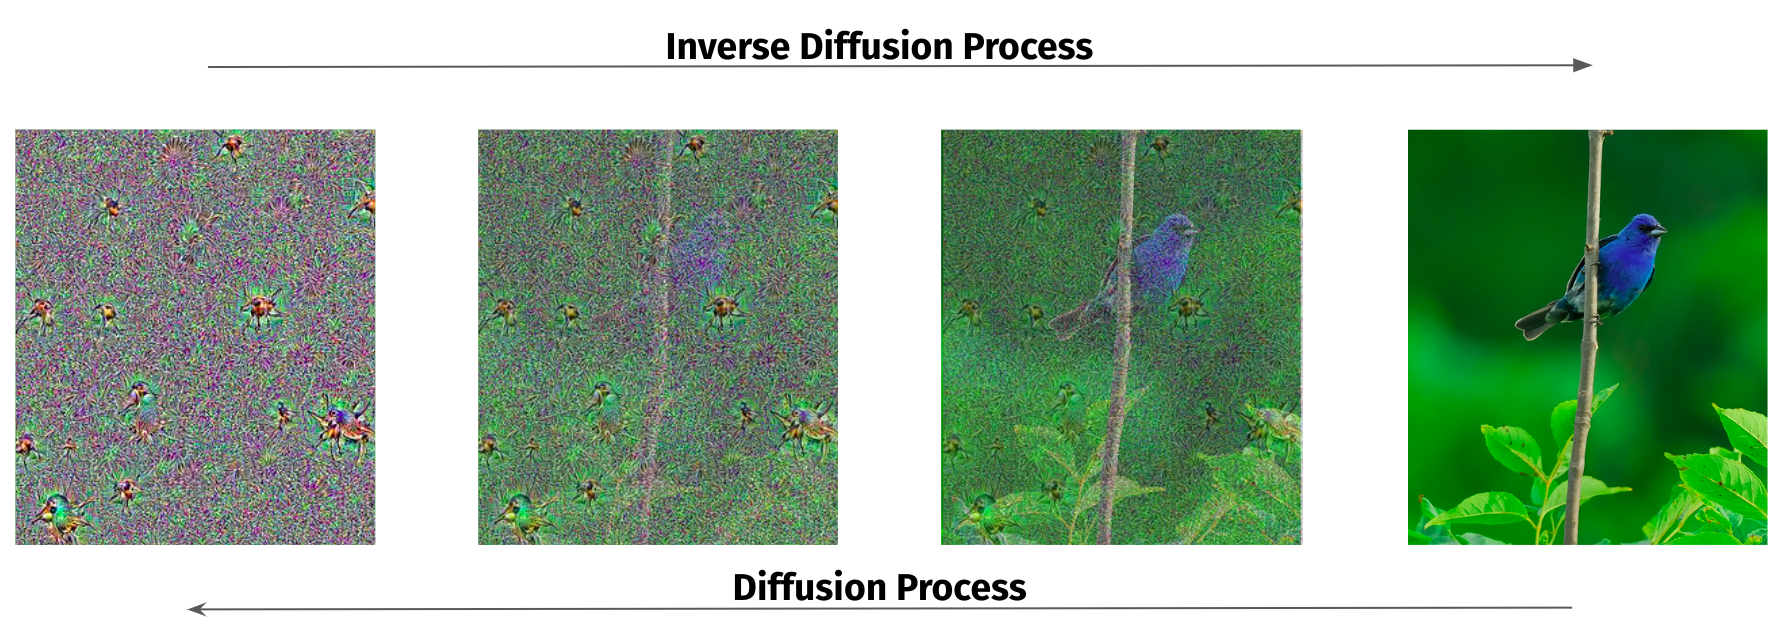
\includegraphics[scale=0.2]{./pic/diffusion_intro.png}
  \end{figure}
\end{frame}
\begin{frame}{Timeline}
\begin{enumerate}
  \item[\bf 2015)] \textit{\ldots Non-equilibrium Thermodynamics}. Sohl-Dickstein
    et al. ICML\vfill
  \item[\bf 2020)] \textit{Denoising Diffusion Probabilistic Models}.
  Ho et al. NeurIPS.\vfill
  \item[\bf 2021)] \textit{Score-Based Generative Modeling Through SDE}. Song et
    al. ICLR.
\end{enumerate}
\end{frame}
\begin{frame}{Deep Unsupervised Learning using Non-Equilibrium Thermodynamics}
  \begin{figure}[h!]
    \centering
    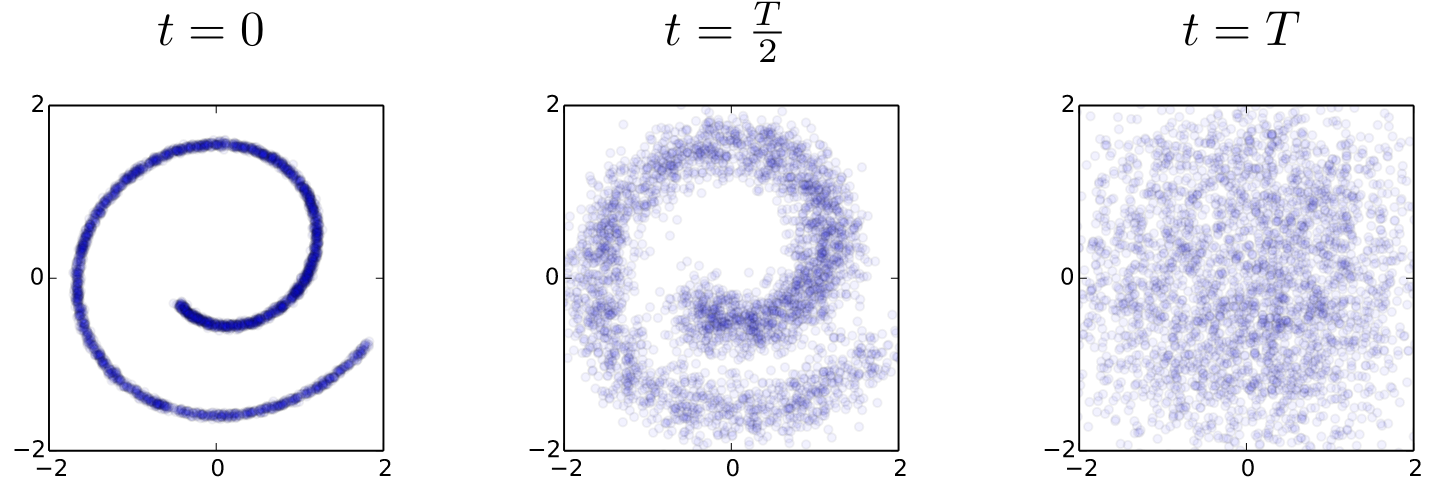
\includegraphics[scale=.23]{./pic/thermodynimc.png}
    \caption{Diffusion process as a \textbf{Markov Chain} with \textbf{Continuous
    State Space} and \textbf{Discrete Time}.\footcite{thermodynamic}}
  \end{figure}
\end{frame}
\begin{frame}{Reminder: Markov Chains with Discrete Time}
\textbf{Informal Definition}\\ 
A sequence of random variables $\xx^{(0)},\xx^{(1)},\cdots,\xx^{(t)},\cdots$,
such that:
\begin{itemize}
  \item $\xx^{(t)}\in S$, where $S$ \textbf{State Space}
  \item The future $\xx^{(t+1)}$ depends on the present $\xx^{(t)}$ 
    but not on the past $\xx^{(t-1)}$
\end{itemize}
  \vfill
  \begin{minipage}[t]{0.5\textwidth}
    \begin{center}
      \textbf{Discrete State Space $S$}
    \end{center}
    \begin{figure}[h!]
      \centering
      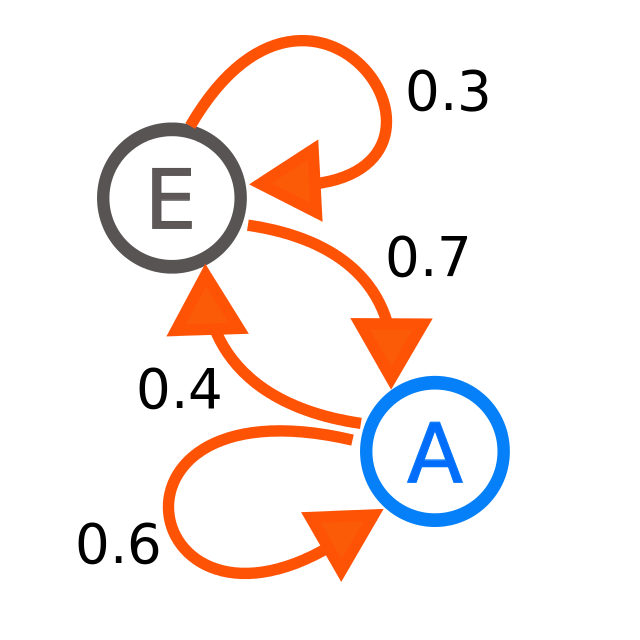
\includegraphics[width=0.5\textwidth, trim=0 0 0
      3cm]{./pic/markov_chain_discrete space.png}\
    \end{figure}
  \end{minipage}\hfill%
  \begin{minipage}[t]{0.5\textwidth}
    \begin{center}
      \textbf{Continuous State Space $S$}
    \end{center}
    \begin{figure}[h!]
      \centering
      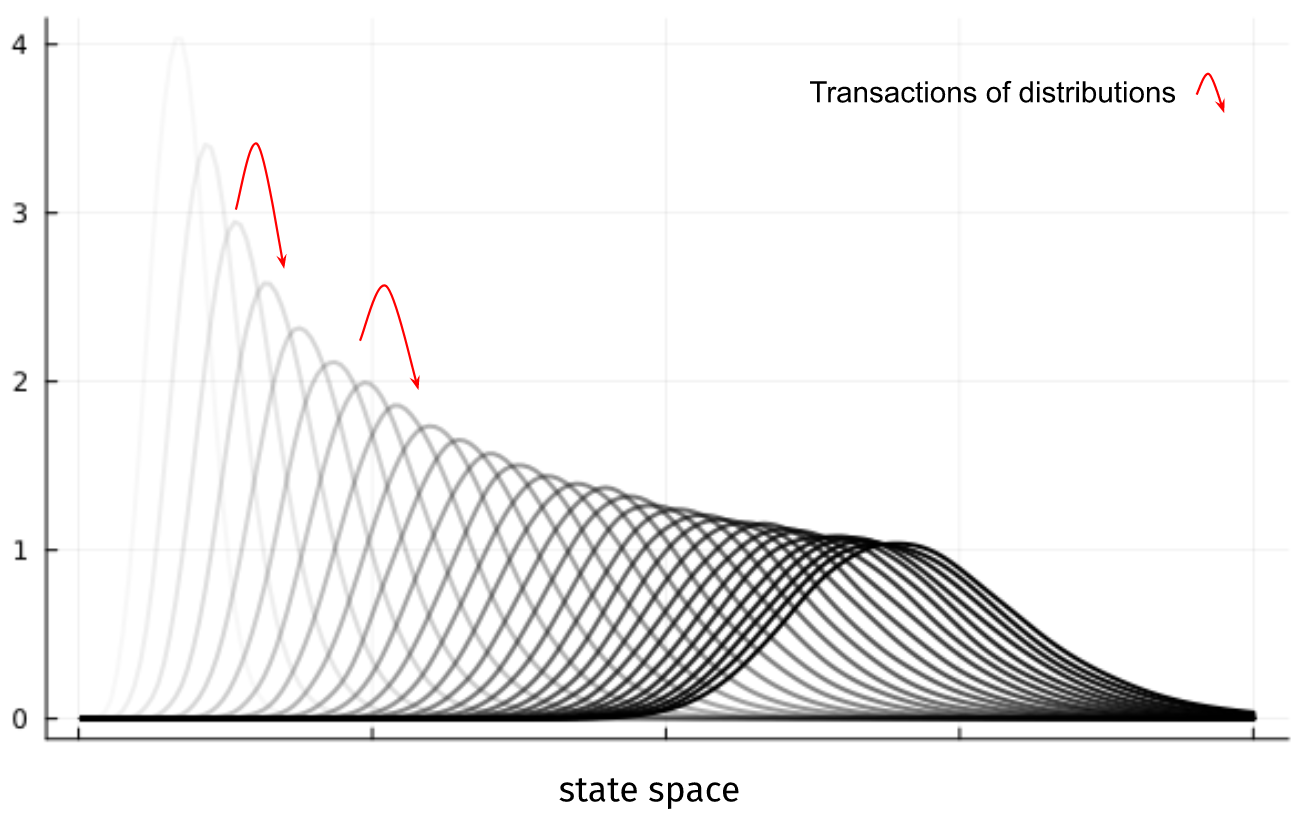
\includegraphics[width=\textwidth, trim=0 0 0
      4cm]{./pic/markov_chain_continous space2.png}
    \end{figure}
  \end{minipage}
\end{frame}
\begin{frame}{Reminder: MCDT with Discrete State Space}
  \begin{minipage}[t]{0.6\textwidth}
    \textbf{Definition}\\
    A sequence $\left\{ \xx^{(t)}\right\}_{t\in\N}
    \subseteq S$, a matrix $P=\left( p_{ij} \right)$.
    \vspace{1cm}
    \begin{itemize}
      %\item %\textbf{Discrete Time Property}\\
      %\(
      %  \xx^{(0)},\,\xx^{(1)},\cdots,\xx^{(t)},\cdots 
      %\)
      %\item \textbf{Discrete Space}\\
      \item \textbf{Discrete state space}: \(
        S=\left\{ s_0,\cdots,s_n,\cdots \right\}
      \) 
      \vspace{1cm}
    \item \textbf{Markov Property:} $\xx^{(t+1)}$ not dep. $\xx^{(0)},\cdots,\xx^{(t-1)}$.
      \vspace{1cm}

    \item \textbf{Transaction Matrix}: \(
        \Ph\left( \xx^{(t+1)}=s_j \vert \xx^{(t)}=s_i\right)=p_{ij}
      \)
%      \(
%        \Ph\left( \xx^{(t+1)}\in A\,\vert\, \xx^{(0)},\ldots,\xx^{(t)}
%        \right)=\Ph\left(\xx^{(t+1)}\in A\,\vert\,\xx^{(t)} \right)
%      \)
    \end{itemize}
  \end{minipage}\hfill%
  \onslide<2>{%
  \begin{minipage}[t]{0.3\textwidth}
    \textbf{$P$ is a stochastic matrix!}\\
    \[
      \forall i,\quad \sum_{j\in\N}p_{ij}=1
    \]
    \begin{figure}[h!]
      \centering
      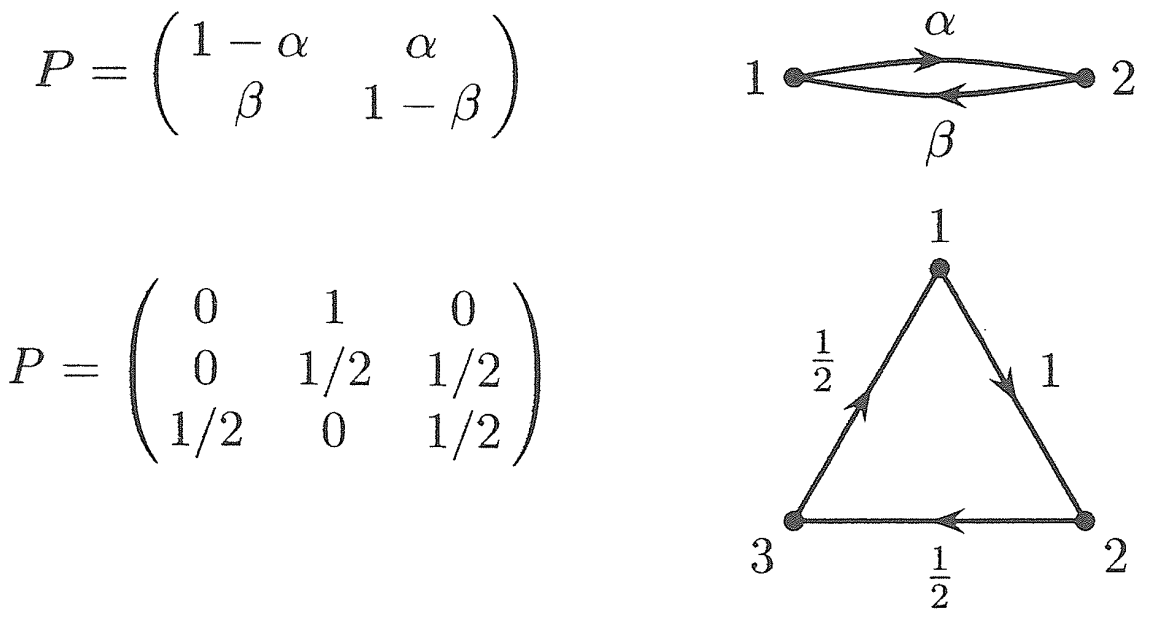
\includegraphics[width=\textwidth]{./pic/mcdt_discrete_space.png}
    \end{figure}
  \end{minipage}
  }
\end{frame}
\begin{frame}{Reminder: DTMC with Continuous State Space}
  Let assume $\xx,\yy\in S$ where $S$ continuous state space (e.g.
  $S=\R^d$).\\
  \vfill
  \textbf{Joint Distribution} $p(\xx,\yy)$
  \[
    \Ph\left( \xx\in A\,\vert\,\yy\in B \right)=
    \int_A\int_B p\left( \xx,\yy \right)\,d\xx\,d\yy
  \]

  \textbf{Transactional Kernel} $p(\xx\,\vert\,\yy)$
  \[
    p\left( \xx,\yy \right) = p(\xx\,\vert\,\yy)\,p\left( \yy \right)
  \]
  \textbf{Marginal Distribution} $p(\xx)$
  \[
    p\left( \xx \right)=\int_S p\left( \xx,\yy \right)\,d\yy = \int_S
    p(\xx\,\vert\,\yy)\,p\left( \yy\right)\,d\yy 
  \]

\end{frame}
\begin{frame}{Forward Diffusion Process}
  \begin{center}
    ``Adding noise to data\ldots''
  \end{center}
  \begin{itemize}
    \item \textbf{Data Distribution}: $\xx^{(0)}\sim q$
      \hfill\onslide<2->{{\color{red} Not Analytic!!}}
    \item \textbf{Transaction Kernel}: $q\left( \xx^{(t)}\,\vert\,\xx^{(t-1)}
      \right)=\NN\left( \xx^{(t)};\sqrt{1-\beta_t}\xx^{(t-1)}; \beta_t I \right)$
    \item \textbf{Variance Scheduler}: $\beta_1,\cdots,\beta_T\in\left(
      0,1\right]$ \hfill\onslide<2->{{\color{red} $\beta_T=1$}}

  \end{itemize}
  \begin{figure}[h!]
    \centering
    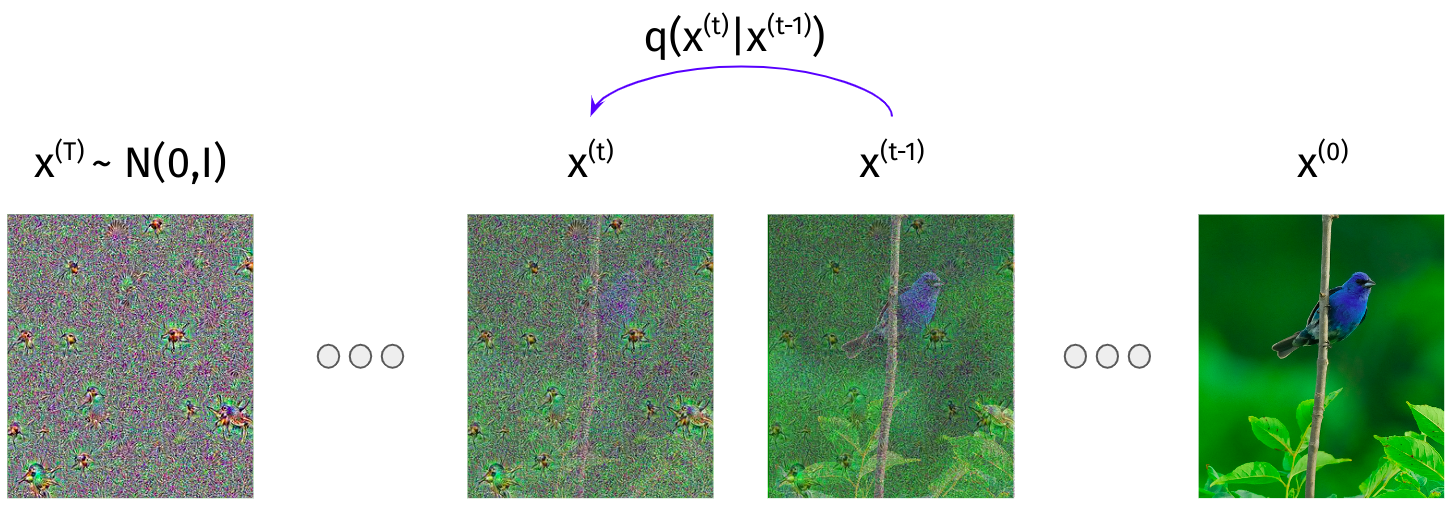
\includegraphics[width=0.75\textwidth]{./pic/forward-diffusion.png}
  \end{figure}
\end{frame}
\begin{frame}{Forward Diffusion Process: Explicit Representation}
  \[
    \xx^{(t)}=\sqrt{1-\beta_t}\,\xx^{(t-1)} +
    \sqrt{\beta_t}\,\varepsilonb_t,\quad
    \varepsilonb_t\sim\NN(0,I)
  \]
  \begin{block}{Observation: Many small noisy steps $\approx$ Large Noisy
    step}
    \[
      \xx^{(t)} = \sqrt{1-\alpha_t}\, \xx^{(0)} + \sqrt{\alpha_t}
      \varepsilonb,\quad \varepsilonb\sim\NN(0,I)
    \]
    where
    \[
      \alpha_t = 1-\prod_{i=0}^t(1-\beta_i)
    \]
  \end{block}
\end{frame}
\begin{frame}{Forward Diffusion Process: Distribution Representation}
  \begin{center}
    Markov property allows breaking up distributional Representation\ldots
  \end{center}
  \begin{equation}
    \begin{aligned}
    q(\xx^{(0)},\ldots,\xx^{(T)}) &= q\left( \xx^{(T)}\,|\,
      \xx^{(0)},\ldots,\xx^{(T-1)} \right)\,q\left(
      \xx^{(0)},\ldots,\xx^{(T-1)} \right)\\
      \pause
      &= q\left(\xx^{(T)}\,\vert\, \xx^{(T-1)}\right) q\left(
      \xx^{(0)},\ldots,\xx^{(T-1)} \right)\\
      &\vdots\\
    \end{aligned}
  \end{equation}
  \pause
  \begin{block}{Distributional Representation}
    \[
      q(\xx^{(0)},\ldots,\xx^{(T)})= q(\xx^{(0)})\prod_{t=1}^T q\left(
          \xx^{(t)}\,\vert\,\xx^{(t-1)}
        \right)
    \]
  \end{block}
\end{frame}
\begin{frame}{Reverse Diffusion Process}
  \begin{figure}[h!]
    \centering
    \includegraphics<1>[clip, width=\textwidth, trim=0 6.3cm 0 4.5cm]{./pic/reverse-diffusion.png}%
    \includegraphics<2>[width=\textwidth,trim=0 6.3cm 0 4.5cm]{./pic/reverse-diffusion.png}
  \end{figure}
\end{frame}
\begin{frame}{Reverse Diffusion Process}
  \begin{minipage}[t]{0.45\textwidth}
    \begin{center}
      \bf 
      Forward Diffusion Process
    \end{center}
    \begin{equation*}
      \begin{aligned}
        q(\xx^{(0)}) &\quad\mbox{Data Distribution}\\
        q(\xx^{(0\ldots T)})&= q(\xx^{(0)})\prod_{t=1}^T q\left(
          \xx^{(t)}\,\vert\,\xx^{(t-1)}\right)\\
      \end{aligned}
    \end{equation*}
  \end{minipage}\hfill%
  \begin{minipage}[t]{0.45\textwidth}
    \begin{center}
      \bf 
      Reverse Diffusion Process
    \end{center}
    \begin{equation*}
      \begin{aligned}
        q(x^{(T)}) &= \NN(0,I)\\
          q(\xx^{(0\ldots T)})&= q(\xx^{(T)})\prod_{t=1}^T q\left(
          \xx^{(t-1)}\,\vert\,\xx^{(t)}\right)
      \end{aligned}
    \end{equation*}
  \end{minipage}
  \pause
  \begin{block}{Theorem. Reverse of Gaussian DP is $\approx$ Gaussian DP\footcite{thermodynamic}}
    If $|\beta_i-\beta_{i+1}|\approx 0$, i.e. diffusion \textbf{slow
    enough}, then% $q\left( \xx^{(t)}\,\vert\,\xx^{(t-1)} \right)=\NN\left( \xx^{(t)};\sqrt{1-\beta_t}\xx^{(t-1)}; \beta_t I \right)$ is such that
    \[
      q(\xx^{(t-1)}\,\vert\, \xx^{(t)}) 
      \approx \NN\left(\xx^{(t-1)};\,\onslide<3->{\tikzmarkin{z1}} 
        \mub_\theta\onslide<3->{\tikzmarkend{z1}}\left(
        \xx^{(t)},t \right),\,
        \onslide<3->{\tikzmarkin{z2}}\Sigmab_\theta\onslide<3->{\tikzmarkend{z2}}\left(
    \xx^{(t)},t \right)\right)
    \]
  \end{block}
  \onslide<3->{\tikzmarkin{b} Mean $\mub_\theta$ and covariance
  $\Sigmab_\theta$ have to be learned!!\tikzmarkend{b}}
\end{frame}
\begin{frame}{Visualization of Diffusion Process: 2D dimensional case}
  \begin{figure}[h]
    \centering
    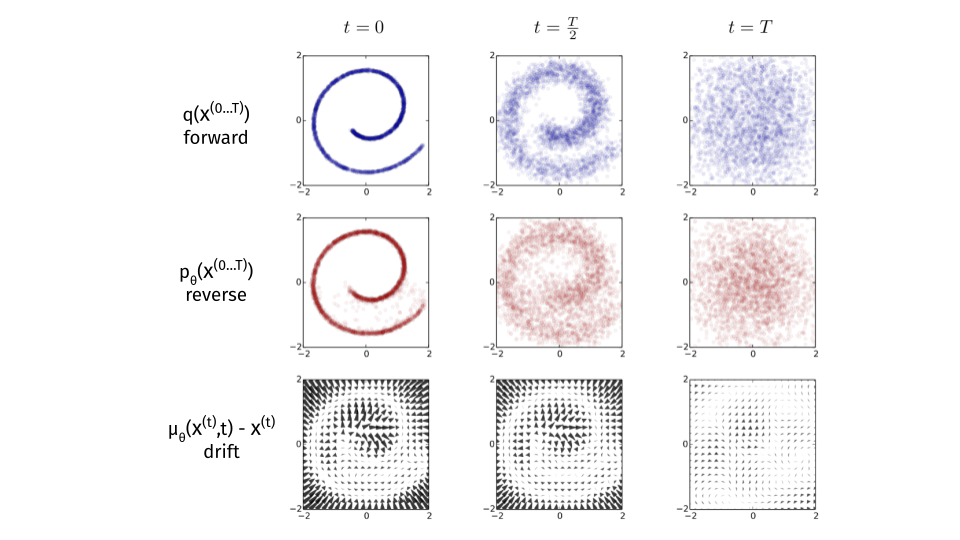
\includegraphics[width=0.75\textwidth]{./pic/summary-forw-reverse.png}\footcite{thermodynamic}
  \end{figure}
\end{frame}
\begin{frame}{Training of $\mub_\theta$ and  $\Sigmab_\theta$}
  \begin{minipage}[t]{0.45\textwidth}
    \begin{center}
      \bf Aim
    \end{center}
    Seach for the best parameters $\theta$ 
    \[
      q(\xx^{(0)}) \approx p_\theta(\xx^{(0)})
    \]
      where $\xx^{(0)}\,\cdots,\,\xx^{(T)}$ diffusion process
      \begin{block}{Estimated Reverse Process}
    \[
      \small
      \begin{aligned}
        & p_\theta(\xx^{(T)}) = \NN\left( \xx^{(T)}; 0, I \right)\\
        & p_\theta(\cdot\,\vert\, \xx^{(t)})=
        \NN\left(\mub_\theta\left(\xx^{(t)},t \right),
          \Sigmab_\theta\left(\xx^{(t)},t \right)\right)
      \end{aligned}
    \]
  \end{block}
  \end{minipage}\hfill%
  \begin{minipage}[t]{0.5\textwidth}
    \onslide<2->{%
    \begin{center}
      \bf Method
    \end{center}
    Minimize the \textit{Kullback–Leibler} Divergence
    \[
      \small
      \onslide<3->{\tikzmarkin{a}(0.1,0.6)(-0.1,-0.5)}%
      D_{KL}(q\,||\,p_\theta):=\int q(\xx^{(0)})\log\left(
      \frac{q(\xx^{(0)})}{p_\theta(\xx^{(0)})}\right)\,d \xx^{(0)}\\
      \onslide<3->{\tikzmarkend{a}}
    \]
      \begin{center}
        \onslide<3->{%
          \textbf{Easy??}\\
        }
        \onslide<4->{%
          \begin{minipage}[t]{0.45\textwidth}
            \vspace{1cm}
            \tikzmarkin{b} \noindent \textbf{No.} $q(\xx^{(0)})$ is analytically
          intractable!!\tikzmarkend{b}
        \end{minipage}\hspace{0.5cm}%
        \begin{minipage}[t]{0.35\textwidth}
          \begin{figure}[h]
            \centering
            \includegraphics<4->[width=\textwidth]{./pic/sample.png}
          \end{figure}
        \end{minipage}
        }
      \end{center}
    }
  \end{minipage}
\end{frame}
\begin{frame}{Training of $\mub_\theta$ and  $\Sigmab_\theta$}
  \begin{center}
    \textbf{Aim: Deduce a tractable loss function}
  \end{center}
    \[
      \tikzmarkin{a1}(0.1,0.6)(-0.1,-0.5)D_{KL}(q\,||\,p_\theta):=\int q(\xx^{(0)})\log\left(
      \frac{q(\xx^{(0)})}{p_\theta(\xx^{(0)})}\right)\,d
      \xx^{(0)}\tikzmarkend{a1}
    \]
    \vfill
    \pause
    \begin{center}
      \bf
      Semplification I: Minimize the Cross Entropy
    \end{center}
    \[
    D_{KL}\left( q(\xx^{(0)})||p_\theta(\xx^{)0)} \right) =
    \only<2>{\int q(\xx^{(0)})\log(q(\xx^{(0)})\,d\xx^{(0)}+
      \int-q(\xx^{(0)})\log(p_\theta(\xx^{(0)}))\,d\xx^{(0)}}
    \only<3->{\underbrace{\int q(\xx^{(0)})\log(q(\xx^{(0)})\,d\xx^{(0)}}_{-\Hh\left(
      q(\xx^{(0)}\right)} + 
    \underbrace{\int-q(\xx^{(0)})\log(p_\theta(\xx^{(0)}))\,d\xx^{(0)}}_{L_{CE}(p_\theta)}}
    \]
\end{frame}
\section{Broader Impacts}
\begin{frame}{CLIP Model}
  \begin{center}
    \it
    ``We also found discrepancies across gender and race for people
    categorized into the ‘crime’ and ‘non-human’
    categories\ldots''\footcite{clip}
  \end{center}
\end{frame}
{%
  \setbeamercolor{background canvas}{bg=black!10!white}
  \setbeamertemplate{background}{%
  \begin{picture}(300,240)
    \hspace{0.9cm}
    
\includegraphics[scale=0.35]{pic/tecip_logo-ENG.png}
    \hspace{0.5cm}
    
\includegraphics[scale=0.17]{pic/dipe.png}
    \hspace{0.5cm}
    
\includegraphics[scale=0.085]{pic/logoretis.png}
  \end{picture}}
\begin{frame}{}
  \textbf{\Huge Thanks for the attention}\\
  \vspace{20pt}
  \begin{minipage}[h]{0.6\textwidth}
  {\large\bf Fabio Brau}
  \vspace{5pt}
  \begin{itemize}
    \item[\faUniversity] {\bf Scuola Superiore Sant'Anna, Pisa}
    \item[\Letter] \texttt{fabio.brau@santannapisa.it}
    \item[\faGlobe] \href{http://retis.santannapisa.it/~f.brau/}{\tt %
                    retis.santannapisa.it/\textasciitilde f.brau}
    \item[\faLinkedin]
      \href{https://www.linkedin.com/in/fabio-brau}{\tt%
        linkedin.com/in/fabio-brau}
  \end{itemize}
  \end{minipage}
\end{frame}
}
\appendix
\section{Proof Details}
\begin{frame}{Proof of Explicit Representation of Forward Diffusion Process}
  Let us proceeding by induction by assuming 
  $\xx^{(t)} = \sqrt{1-\alpha_t}\, \xx^{(0)} + \sqrt{\alpha_t}\,\varepsilonb$
  where $\varepsilonb\sim\NN(0,I)$ and where $\alpha_t =
  1-\prod_{i=0}^t(1-\beta_i)$. 
  \begin{equation}
    \begin{aligned}
      \xx^{(t+1)} &=  \sqrt{1-\beta_{t+1}}\, \xx^{(t)} +
      \sqrt{\beta_{t+1}}\,\varepsilonb_{t+1}\\
      &=\sqrt{1-\beta_{t+1}}\, \left(
      \sqrt{1-\alpha_t}\, \xx^{(0)} + \sqrt{\alpha_t}\,\varepsilonb\right) +
      \sqrt{\beta_{t+1}}\,\varepsilonb_{t+1}\\
      &= \sqrt{\left( \prod_{i=0}^{t+1}(1-\beta_i) \right)}\xx^{(0)} +
      \sqrt{(1-\beta_{t+1})\alpha_t+\beta_{t+1}}\,\tilde\varepsilonb
    \end{aligned}
  \end{equation}
    where the last term of the summation is obtained by observing that, since
    $\sqrt{(1-\beta_{t+1})\alpha_t}\,\varepsilonb$ and $\sqrt{\beta_{t+1}}\,\varepsilonb_{t+1}$ 
      are independent, then the variance of their sum (that still has a
      gaussian distribution) is given by
      $(1-\beta_{t+1})\alpha_t+ \beta_{t+1}$.
\end{frame}
\end{document}
\begin{frame}{Markov Chains with Discrete Time}
\textbf{Definition}\\ 
  A sequence of random variables $\left\{ \xx^{(t)}\right\}_{t\in\TT}
  \subseteq S$, such that the future $\xx^{(t+1)}$ depends on
  the present $\xx^{(t)}$ but not on the past $\xx^{(t-1)}$.\\
  \begin{itemize}
    \item \textbf{Discrete Time Property}\\
      \(
        \xx^{(0)},\,\xx^{(1)},\cdots,\xx^{(t)},\cdots 
      \)
    \item \textbf{Markov Property}\\
      \(
        \Ph\left( \xx^{(t+1)}\in A\,\vert\, \xx^{(0)},\ldots,\xx^{(t)}
        \right)=\Ph\left(\xx^{(t+1)}\in A\,\vert\,\xx^{(t)} \right)
      \)
  \end{itemize}
  \vfill
  \begin{minipage}[t]{0.4\textwidth}
    \begin{center}
      \textbf{Discrete State Space $S$}
    \end{center}
  \end{minipage}\hfill%
  \begin{minipage}[t]{0.4\textwidth}
    \begin{center}
      \textbf{Continuous State Space $S$}
    \end{center}
  \end{minipage}
\end{frame}
    \[
    D_{KL}\left( q(\xx^{(0)})||p_\theta(\xx^{)0)} \right) =
    \only<2>{\int q(\xx^{(0)})\log(q(\xx^{(0)})\,d\xx^{(0)}+
      \int-q(\xx^{(0)})\log(p_\theta(\xx^{(0)}))\,d\xx^{(0)}}
    \only<3->{\underbrace{\int q(\xx^{(0)})\log(q(\xx^{(0)})\,d\xx^{(0)}}_{-\Hh\left(
      q(\xx^{(0)}\right)} + 
    \underbrace{\int-q(\xx^{(0)})\log(p_\theta(\xx^{(0)}))\,d\xx^{(0)}}_{L_{CE}(p_\theta)}}
    \]
